\documentclass[12pt, a4paper]{article}
\usepackage{tikz}


% Title Page
\title{Evolving Tower-Destroying Robots\\\normalsize An Exploration into Scaffolded Learning}
\author{Ryan Boldi}


\begin{document}
\maketitle
\tableofcontents
\newpage
\section{Goals}
We do not teach linear algebra to 6 year olds due to the fact that they do not have sufficient educational \emph{scaffolding} to grasp such a bizarre concept. My goal was to see whether or not this also applies to a robot evolving to do a certain task.\par 
The robot's task is to destroy a tower that starts a specific distance away from it:\par
\vspace{-10pt}
\begin{figure}[h]
\begin{center}
	\centering
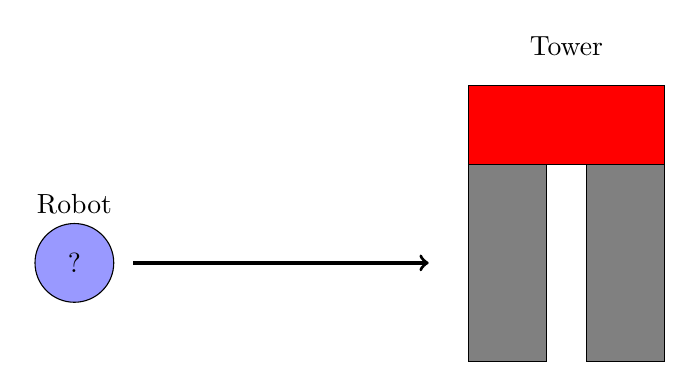
\begin{tikzpicture}
\filldraw[fill=blue!40!white](0,1.25) circle (5mm);
\node[] at (0,1.25) {?};
\node[] at (0,2) {Robot};
\draw [->, very thick] (0.75, 1.25) -- (4.5,1.25);
\filldraw[fill=gray] (5,0) rectangle (6,2.5);
\filldraw[fill=gray](6.5,0) rectangle (7.5,2.5);
\filldraw[fill=red] (5,2.5) rectangle (7.5,3.5);
\node[] at (6.25,4) {Tower};
\end{tikzpicture}
\caption{Diagram demonstrating the robot's task.}
\end{center}
\end{figure}
\vspace{-10pt}
To scaffold the learning of the robot, I planned to start the tower close to the robot, and slowly move it farther and farther away over the course of many generations. This will continue until the tower is at the goal distance from the robot. These are environmental changes that starts the robot with an easy task, waits for the task to be complete, then makes the task slightly harder. This process is repeated until the robot has mastered the most difficult goal task.\par
My goal was to experiment with this process, seeing whether or not it actually improved the speed of solution discovery, or quality of the solutions themselves.

\section{Implementation}
I started by creating the robot. It was based on a simple quadruped, but with 2 added arms to make destroying the tower easier.
The block colored in red is to be my 'fall detector'. If this block comes into contact with the ground, we will count this tower as "Fallen".
\section{Results}
\section{Reflection}

\end{document}          
